\chapter{Methodological Framework}\label{ch:methodology_approach}

The methodological framework employed in this thesis is grounded in the V-model as established by the \gls{incose} \autocite{INCOSE2015} for project development. The V-model offers a rigorous and structured method that ensures all project facets are considered, facilitating timely and budget-compliant completion. This is achieved through a comprehensive development process, enabling clear validation and verification of initial requirements at every stage.

The methodology is segmented into seven key components which can be summarized as follows:

\begin{enumerate}
  \item \textbf{Identification of User Requirements}: A detailed analysis of the problem statement is conducted to identify the primary issues and potential solutions. Moreover, the user requirements are defined to ensure that the proposed solution aligns with the objectives of the project.

  \item \textbf{System Design}: The system architecture is developed based on the user requirements, ensuring that the proposed solution is feasible and aligns with the project's objectives. This phase includes a detailed overview of the system components and their interconnections. Requirements are formulated to satisfy the previously defined solution requirements. This phase includes a high-level overview of the components of the proposed solution, the justification for their selection, and the interconnections among them.

  \item \textbf{Component Design}: Building upon the high-level architecture of the solution, a more detailed approach is outlined for each component, taking into account their specific power and data transmission needs. This culminates in a comprehensive architecture of the solution. Furthermore, a detailed overview of the components is provided, including the rationale for their selection and the interconnections among them.

  \item \textbf{Implementation}: The proposed solution is implemented and manufactured utilizing available tools while simultaneously integrating the necessary electrical components. This phase includes a detailed description of the implementation process, including the tools and materials used, as well as the integration of electrical components. The development of software and hardware components is also detailed.

  \item \textbf{Component Testing}: The functionality of each component is verified in a standalone mode, with detailed information provided regarding the verification process.

  \item \textbf{System Testing}: The methodology for conducting flight tests and subsequent analyses is elaborated. System integration is performed by assessing communication between module pairs to ensure that data can be transmitted freely and utilized effectively.

  \item \textbf{Acceptance Testing}: Validation of the initial requirements is conducted to confirm that all solution requirements have been met. This phase also includes preparations for potential future enhancements.
\end{enumerate}

\begin{figure}
  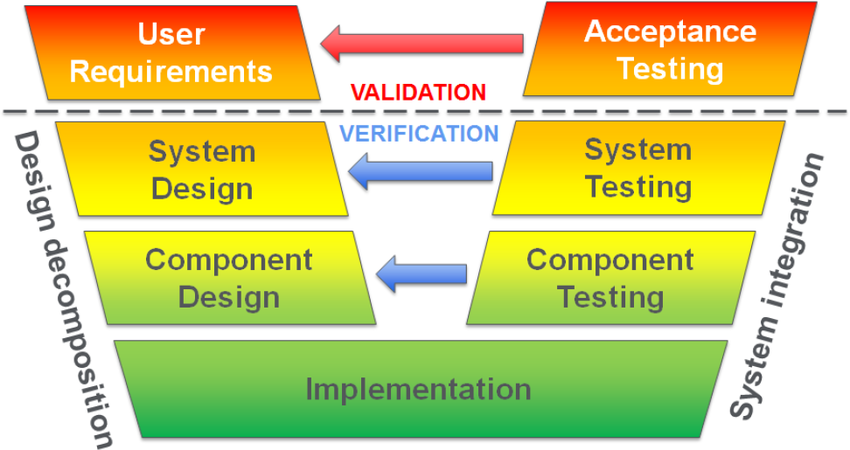
\includegraphics{v_model_methodology.png}
  \caption{Methodological framework based on the V-model from \glsentryshort{incose} with the different stages of the project development process\autocite{ruddle2020vmodel}}\label{fig:v_model_methodology}
\end{figure}

Moreover, a graphical representation of the V-model is provided in \cref{fig:v_model_methodology} to illustrate the methodology's structure and the relationship between the various stages.
